\documentclass[a4paper,12pt]{article} 

% First, we usually want to set the margins of our document. For this we use the package geometry.
\usepackage[top = 2.5cm, bottom = 2.5cm, left = 2.5cm, right = 2.5cm]{geometry} 
\usepackage[T1]{fontenc}
\usepackage[utf8]{inputenc}

% The following two packages - multirow and booktabs - are needed to create nice looking tables.
\usepackage{multirow} % Multirow is for tables with multiple rows within one cell.
\usepackage{booktabs} % For even nicer tables.

% As we usually want to include some plots (.pdf files) we need a package for that.
\usepackage{graphicx} 

% The default setting of LaTeX is to indent new paragraphs. This is useful for articles. But not really nice for homework problem sets. The following command sets the indent to 0.
%\usepackage{setspace}
%\setlength{\parindent}{0in}
\usepackage{indentfirst}

% Package to place figures where you want them.
\usepackage{float}

% The fancyhdr package let's us create nice headers.
\usepackage{fancyhdr}

\usepackage{amsmath,amsthm,amsfonts,tikz}

% To make our document nice we want a header and number the pages in the footer.

\pagestyle{fancy} % With this command we can customize the header style.

\fancyhf{} % This makes sure we do not have other information in our header or footer.

\lhead{\footnotesize Discrete Mathematics(H): Homework 5}% \lhead puts text in the top left corner. \footnotesize sets our font to a smaller size.

%\rhead works just like \lhead (you can also use \chead)
\rhead{\footnotesize Mengxuan Wu} %<---- Fill in your lastnames.

% Similar commands work for the footer (\lfoot, \cfoot and \rfoot).
% We want to put our page number in the center.
\cfoot{\footnotesize \thepage} 

\begin{document}

\thispagestyle{empty} % This command disables the header on the first page. 

\begin{tabular}{p{15.5cm}}
{\large \bf Discrete Mathematics(H)} \\
Southern University of Science and Technology \\ Mengxuan Wu \\ 12212006 \\
\hline
\\
\end{tabular}

\vspace*{0.3cm} %add some vertical space in between the line and our title.

\begin{center}
	{\Large \bf Assignment 5}
	\vspace{2mm}

	{\bf Mengxuan Wu}
		
\end{center}  

\vspace{0.4cm}

\section*{Q.1}

\subsection*{(1)}

$R_1$ is irreflexive, symmetric.

Because for any string $a$, $a$ and $a$ always have letters in common, thus $(a, a) \not\in R_1$.
Thus, $R_1$ is irreflexive, and it can't be reflexive.

Because for any strings $a, b$, if $(a, b) \in R_1$, then $a$ and $b$ have no letter in common.
Then $b$ and $a$ also have no letter in common, thus $(b, a) \in R_1$.
However, $(a,b)$ and $(b,a)$ is both in $R_1$ does not imply $a = b$, for two different strings can have no letter in common.
Thus, $R_1$ is symmetric, and it can't be antisymmetric.

$R_1$ is not transitive.
For strings $a = \text{``A''}$, $b = \text{``B''}$, $c = \text{``A''}$, $(a, b) \in R_1$ and $(b, c) \in R_1$, but $(a, c) \not\in R_1$.

\subsection*{(2)}

$R_2$ is irreflexive, symmetric.

Because for any string $a$, $a$ and $a$ always have the same length, thus $(a, a) \not\in R_2$.
Thus, $R_2$ is irreflexive, and it can't be reflexive.

Because for any strings $a, b$, if $(a, b) \in R_2$, then $a$ and $b$ don't have the same length.
Then $b$ and $a$ also don't have the same length, thus $(b, a) \in R_2$.
However, $(a,b)$ and $(b,a)$ is both in $R_2$ does not imply $a = b$, for two different strings can have different lengths.
Thus, $R_2$ is symmetric, and it can't be antisymmetric.

$R_2$ is not transitive.
For strings $a = \text{``A''}$, $b = \text{``BB''}$, $c = \text{``C''}$, $(a, b) \in R_2$ and $(b, c) \in R_2$, but $(a, c) \not\in R_2$.

\subsection*{(3)}

$R_3$ is irreflexive, antisymmetric and transitive.

Because for any string $a$, $a$ can't be longer than itself, thus $(a, a) \not\in R_3$.
Thus, $R_3$ is irreflexive, and it can't be reflexive.

Because for any strings $a, b$, if $(a, b) \in R_3$, then $a$ is longer than $b$.
Then $b$ can't be longer than $a$, thus $(b, a) \not\in R_3$.
Thus, $R_3$ can't be symmetric.

For any strings $a, b, c$, if $(a, b) \in R_3$ and $(b, a) \in R_3$, then $a$ is longer than $b$ and $b$ is longer than $a$.
However, this is a contradiction.
Then, $(a, b) \in R_3$ and $(b, a) \in R_3$ imply $a = b$ is a tautology.
Thus, $R_3$ is antisymmetric.

For any strings $a, b, c$, if $(a, b) \in R_3$ and $(b, c) \in R_3$, then $a$ is longer than $b$ and $b$ is longer than $c$.
Then, $a$ is longer than $c$, thus $(a, c) \in R_3$.
Thus, $R_3$ is transitive.

\section*{Q.2}

\subsection*{(1)}

$R$ is reflexive. 
For any $a \in \mathbb{R}$, $a - a = 0 \in \mathbb{Q}$. 
So $(a, a) \in R$.

\subsection*{(2)}

$R$ is symmetric. 
For any $a, b \in \mathbb{R}$, if $(a, b) \in R$, then $a - b \in \mathbb{Q}$. So $b - a = -(a - b) \in \mathbb{Q}$. 
So $(b, a) \in R$.

\subsection*{(3)}

$R$ is not antisymmetric. 
For $a = 1$ and $b = 0$, $a - b = 1 \in \mathbb{Q}$ and $b - a = -1 \in \mathbb{Q}$. 
So $(a, b) \in R$ and $(b, a) \in R$. 
But $a \neq b$.

\subsection*{(4)}

$R$ is transitive. 
For any $a, b, c \in \mathbb{R}$, if $(a, b) \in R$ and $(b, c) \in R$, then $a - b \in \mathbb{Q}$ and $b - c \in \mathbb{Q}$. 
Let $\frac{m_1}{n_1} = a - b$ and $\frac{m_2}{n_2} = b - c$, where $m_1, n_1, m_2, n_2 \in \mathbb{Z}$ and $n_1, n_2 \neq 0$. 
Then $a - c = (a - b) + (b - c) = \frac{m_1}{n_1} + \frac{m_2}{n_2} = \frac{m_1n_2 + m_2n_1}{n_1n_2} \in \mathbb{Q}$.
So $(a, c) \in R$.

\section*{Q.3}

\subsection*{(a)}

The number of symmetric relations is $2^{\frac{n^2+n}{2}}$.

\subsection*{(b)}

The number of antisymmetric relations is $3^{\frac{n^2-n}{2}}2^{n}$.

\subsection*{(c)}

The number of irreflexive relations is $2^{n^2-n}$.

\subsection*{(d)}

The number of reflexive and symmetric relations is $2^{\frac{n^2-n}{2}}$.

\subsection*{(e)}

The number of not reflexive nor irreflexive relations is $(2^n - 2)2^{n^2-n}$.

\subsection*{(f)}

The number of reflexive and antisymmetric relations is $3^{\frac{n^2-n}{2}}$.

\subsection*{(g)}

The number of symmetric, antisymmetric and transitive relations is $2^n$.
\section*{Q.4}

No. 
$R^2$ is not irreflexive.

Suppose $R$ is an irreflexive relation on $A$, where $A = \{0, 1\}$ and $R = \{(0, 1), (1, 0)\}$.
Then $R^2 = \{(0, 0), (1, 1)\}$. So $R^2$ is not irreflexive.

\section*{Q.5}

\subsection*{(1)}

Since $R_1$ and $R_2$ are reflexive, then for any $a \in A$, $(a, a) \in R_1$ and $(a, a) \in R_2$.
Therefore, $(a, a) \not\in R_1 \oplus R_2$. So $R_1 \oplus R_2$ is irreflexive.

\subsection*{(2)}

Yes. 
$R_1 \cap R_2$ is reflexive.

Since $R_1$ and $R_2$ are reflexive, then for any $a \in A$, $(a, a) \in R_1$ and $(a, a) \in R_2$.
Therefore, $(a, a) \in R_1 \cap R_2$. So $R_1 \cap R_2$ is reflexive.

\subsection*{(3)}

Yes. 
$R_1 \cup R_2$ is reflexive.

Since $R_1$ and $R_2$ are reflexive, then for any $a \in A$, $(a, a) \in R_1$ and $(a, a) \in R_2$.
Therefore, $(a, a) \in R_1 \cup R_2$. So $R_1 \cup R_2$ is reflexive.

\section*{Q.6}

\subsection*{(1)}

$R$ is an equivalence relation.

\textbf{Reflexive:} 

For any ordered pair $(a, b)$ where $a, b \in \mathbb{Z^+}$, $ab = ba$ is always true, thus $((a, b), (a, b)) \in R$.
Hence, $R$ is reflexive.

\textbf{Symmetric:}

For any ordered pair $(a, b)$, $(c, d)$ where $a, b, c, d \in \mathbb{Z^+}$, if $((a, b), (c, d)) \in R$, then $ad = bc$.
Therefore, $cb = da$, and $((c, d), (a, b)) \in R$.
Hence, $R$ is symmetric.

\textbf{Transitive:}

For any ordered pair $(a, b)$, $(c, d)$, $(e, f)$ where $a, b, c, d, e, f \in \mathbb{Z^+}$, if $((a, b), (c, d)) \in R$ and $((c, d), (e, f)) \in R$, then $ad = bc$ and $cf = de$.
Therefore, $af = \frac{adcf}{dc} = \frac{bcde}{dc} = be$, thus $((a, b), (e, f)) \in R$.
Hence, $R$ is transitive.

\subsection*{(2)}

Let $(a, b) = (1, 2)$, then $2a = b$.
Hence, the equivalence class of $(1, 2)$ is $\{(a, b) | 2a = b \text{ and } a, b \in \mathbb{Z^+}\}$.

\subsection*{(3)}

Each equivalence class is a set of ordered pairs with the same value of $\frac{a}{b}$.

\section*{Q.7}

\subsection*{(1)}

\begin{proof}
$ $

$R$ is an equivalence relation.

\textbf{Reflexive:}

For any tuple $(a, b, c)$ where $a, b, c \in \mathbb{R}$, $(a, b, c) = 1 \cdot (a, b, c)$ and $1 \in \mathbb{R} \backslash \{0\}$.
Hence, $R$ is reflexive.

\textbf{Symmetric:}

For any tuple $(a, b, c)$, $(d, e, f)$ where $a, b, c, d, e, f \in \mathbb{R}$, if $(a, b, c) = k (d, e, f)$ where $k \in \mathbb{R} \backslash \{0\}$.
Then $(d, e, f) = \frac{1}{k} (a, b, c)$, where $\frac{1}{k} \in \mathbb{R} \backslash \{0\}$.
Hence, $R$ is symmetric.

\textbf{Transitive:}

For any tuple $(a, b, c)$, $(d, e, f)$, $(g, h, i)$ where $a, b, c, d, e, f, g, h, i \in \mathbb{R}$, if $(a, b, c) = k_1 (d, e, f)$ and $(d, e, f) = k_2 (g, h, i)$ where $k_1, k_2 \in \mathbb{R} \backslash \{0\}$.
Then $(a, b, c) = k_1 k_2 (g, h, i)$, where $k_1 k_2 \in \mathbb{R} \backslash \{0\}$.
Thus, $(a, b, c) R (g, h, i)$.
Hence, $R$ is transitive.
\end{proof}

\subsection*{(2)}

\begin{equation*}
	[(1,1,1)]_R = \{(1,1,1), (2,2,2), (3,3,3), (4,4,4), \dots\}
\end{equation*}

\begin{equation*}
	[(1,0,3)]_R = \{(1,0,3), (2,0,6), (3,0,9), (4,0,12), \dots\}
\end{equation*}

\subsection*{(3)}

No. Not all equivalence classes have the same cardinality.

\begin{proof}[Disproof]
$ $ 

The equivalence class $[(1, 1, 1)]_R$ has infinite elements, while the equivalence class $[(0, 0, 0)]_R$ has only one element.
\end{proof}

\section*{Q.8}

\begin{proof}
$ $

$T$ is an equivalence relation.

\textbf{Reflexive:}

Since $R$ and $S$ are both reflexive, then for any $a \in A$, $(a, a) \in R$ and $(a, a) \in S$.
Therefore, $(a, a) \in R \cap S$.
Hence, $T$ is reflexive.

\textbf{Symmetric:}

For any $a, b \in A$, if $(a, b) \in T$, then $(a, b) \in R$ and $(a, b) \in S$.
Because $R$ and $S$ are both symmetric, then $(b, a) \in R$ and $(b, a) \in S$.
Therefore, $(b, a) \in R \cap S$.
Hence, $T$ is symmetric.

\textbf{Transitive:}

For any $a, b, c \in A$, if $(a, b) \in T$ and $(b, c) \in T$, then $(a, b), (b, c) \in R$ and $(a, b), (b, c) \in S$.
Because $R$ and $S$ are both transitive, then $(a, c) \in R$ and $(a, c) \in S$.
Thus, $(a, c) \in R \cap S$.
Hence, $T$ is transitive.
\end{proof}

\section*{Q.9}

\subsection*{(a)}

Yes. 
$(\mathbb{R}, =)$ is a partially ordered set and $=$ is a partial order.

\textbf{Reflexive:}

For any $a \in \mathbb{R}$, $a = a$.
Therefore, $(a, a) \in R$.
Hence, $=$ is reflexive.

\textbf{Antisymmetric:}

For any $a, b \in \mathbb{R}$, if $(a, b) \in R$ and $(b, a) \in R$, then $a = b$ and $b = a$.
Therefore, $(a, b)$ and $(b, a)$ imply $a = b$.
Hence, $=$ is antisymmetric.

\textbf{Transitive:}

For any $a, b, c \in \mathbb{R}$, if $(a, b) \in R$ and $(b, c) \in R$, then $a = b$ and $b = c$.
Therefore, $a = c$, thus $(a, c) \in R$.
Hence, $=$ is transitive.

\subsection*{(b)}

No.
$(\mathbb{R}, <)$ is not a partially ordered set.

This is because $<$ is not reflexive.
For any $a \in \mathbb{R}$, $a < a$ is false.

\subsection*{(c)}

Yes.
$(\mathbb{R}, \leq)$ is a partially ordered set and $\leq$ is a partial order.

\textbf{Reflexive:}

For any $a \in \mathbb{R}$, $a \leq a$.
Therefore, $(a, a) \in R$.
Hence, $\leq$ is reflexive.

\textbf{Antisymmetric:}

For any $a, b \in \mathbb{R}$, if $(a, b) \in R$ and $(b, a) \in R$, then $a \leq b$ and $b \leq a$.
Therefore, $a = b$.
Hence, $\leq$ is antisymmetric.

\textbf{Transitive:}

For any $a, b, c \in \mathbb{R}$, if $(a, b) \in R$ and $(b, c) \in R$, then $a \leq b$ and $b \leq c$.
Therefore, $a \leq c$, thus $(a, c) \in R$.
Hence, $\leq$ is transitive.

\subsection*{(d)}

No.
$(\mathbb{R}, \neq)$ is not a partially ordered set.

This is because $\neq$ is not reflexive.
For any $a \in \mathbb{R}$, $a \neq a$ is false.

\section*{Q.10}

\subsection*{(a)}

\begin{proof}
$ $

$\preceq$ is a partial order.

\textbf{Reflexive:}

For any function $f : \mathbb{R} \rightarrow \mathbb{R}$, $f(x) \leq f(x)$ is true for any $x \in \mathbb{R}$.
Hence, $\preceq$ is reflexive.

\textbf{Antisymmetric:}

For any functions $f, g : \mathbb{R} \rightarrow \mathbb{R}$, if $f \preceq g$ and $g \preceq f$, then $f(x) \leq g(x)$ and $g(x) \leq f(x)$ for any $x \in \mathbb{R}$.
Therefore, $f(x) = g(x)$ for any $x \in \mathbb{R}$.
Hence, $\preceq$ is antisymmetric.

\textbf{Transitive:}

For any functions $f, g, h : \mathbb{R} \rightarrow \mathbb{R}$, if $f \preceq g$ and $g \preceq h$, then $f(x) \leq g(x)$ and $g(x) \leq h(x)$ for any $x \in \mathbb{R}$.
Therefore, $f(x) \leq h(x)$ for any $x \in \mathbb{R}$, thus $f \preceq h$.
Hence, $\preceq$ is transitive.
\end{proof}

\subsection*{(b)}

\begin{proof}[Disproof]
$ $

$\preceq$ is not a total order.

Let $f(x) = x$ and $g(x) = -x$ for any $x \in \mathbb{R}$.
Then $f \preceq g$ and $g \preceq f$ are both false.
\end{proof}

\section*{Q.11}

\subsection*{(a)}

Yes.
$\preceq$ is reflexive.

For any positive integer $a$, let $m_a$ be the sum of distinct prime factors of $a$.
Then obviously $m_a \leq m_a$, thus $a \preceq a$.
Hence, $\preceq$ is reflexive.

\subsection*{(b)}

No.
$\preceq$ is not antisymmetric.

For integer 2 and 4, the sum of prime factors are both 2.
Then, $(2,4), (4,2) \in R$.
However, $2 \neq 4$.
Hence, $\preceq$ is not antisymmetric.

\subsection*{(c)}

Yes.
$\preceq$ is transitive.

For any positive integers $a, b, c$, if $a \preceq b$ and $b \preceq c$, then $m_a \leq m_b$ and $m_b \leq m_c$.
Therefore, $m_a \leq m_c$, thus $a \preceq c$.
Hence, $\preceq$ is transitive.

\section*{Q.12}

\subsection*{(1)}

\begin{proof}
$ $

$R$ is a partial ordering.

\textbf{Reflexive:}

For a tuple $(a,b,c)$ where $a, b, c \in \mathbb{N}$, $2^a3^b5^c \leq 2^a3^b5^c$ is always true.
Hence, $R$ is reflexive.

\textbf{Antisymmetric:}

For tuples $(a,b,c)$, $(d,e,f)$ where $a, b, c, d, e, f \in \mathbb{N}$, if $2^a3^b5^c \leq 2^d3^e5^f$ and $2^d3^e5^f \leq 2^a3^b5^c$, then $2^a3^b5^c = 2^d3^e5^f$.
By the fundamental theorem of arithmetic, $a = d$, $b = e$ and $c = f$.
Therefore, $(a,b,c) = (d,e,f)$.
Hence, $R$ is antisymmetric.

\textbf{Transitive:}

For tuples $(a,b,c)$, $(d,e,f)$, $(g,h,i)$ where $a, b, c, d, e, f, g, h, i \in \mathbb{N}$, and $(a,b,c) R (d,e,f)$ and $(d,e,f) R (g,h,i)$, then $2^a3^b5^c \leq 2^d3^e5^f$ and $2^d3^e5^f \leq 2^g3^h5^i$.
Therefore, $2^a3^b5^c \leq 2^g3^h5^i$, thus $(a,b,c) R (g,h,i)$.
Hence, $R$ is transitive.
\end{proof}

\subsection*{(2)}

$(1,1,1)$ and $(2,2,2)$ are comparable elements.

There is no incomparable elements.

\subsection*{(3)}

To find the least upper bound for $(5,0,1)$ and $(1,1,2)$, we need to find the smallest number $2^a3^b5^c$ that is greater than or equal to both $2^53^05^1 = 160$ and $2^13^15^2 = 150$.
Hence, the least upper bound is $(5,0,1)$.

Similarly, we can find the greatest lower bound for $(5,0,1)$ and $(1,1,2)$, which is $(1,1,2)$.

\subsection*{(4)}

The minimal element is $(0,0,0)$.

There is no maximal element.

\section*{Q.13}

$(\mathbb{Z} \times \mathbb{Z}, \preceq)$ is a partially ordered set.

\textbf{Reflexive:}

For any $(a, b) \in \mathbb{Z} \times \mathbb{Z}$, $(a, b) = (a, b)$ is always true.
Therefore, $(a, b) \preceq (a, b)$.
Hence, $\preceq$ is reflexive.

\textbf{Antisymmetric:}

For any $(a, b), (c, d) \in \mathbb{Z} \times \mathbb{Z}$, suppose $(a, b) \preceq (c, d)$ and $(c, d) \preceq (a, b)$.
If $(a, b) \neq (c, d)$, then the two relationships above would be equivalent to $a^2 + b^2 < c^2 + d^2$ and $c^2 + d^2 < a^2 + b^2$, which is a contradiction.
Therefore, $(a, b) = (c, d)$.
Hence, $\preceq$ is antisymmetric.

\textbf{Transitive:}

For any $(a, b), (c, d), (e, f) \in \mathbb{Z} \times \mathbb{Z}$, suppose $(a, b) \preceq (c, d)$ and $(c, d) \preceq (e, f)$.
If $(a, b) \preceq (c, d)$ is equivalent to $a^2 + b^2 < c^2 + d^2$, then $a^2 + b^2 < c^2 + d^2 \leq e^2 + f^2 \rightarrow a^2 + b^2 < e^2 + f^2$.
Therefore, $(a, b) \preceq (e, f)$.
If $(c, d) \preceq (e, f)$ is equivalent to $c^2 + d^2 < e^2 + f^2$, we can get the same result as shown above.
If $(a, b) \preceq (c, d)$ is equivalent to $(a,b) = (c,d)$ and $(c, d) \preceq (e, f)$ is equivalent to $(c,d) = (e,f)$, then $(a,b) = (e,f)$.
Therefore, $(a, b) \preceq (e, f)$.
Hence, $\preceq$ is transitive.

\textbf{Hasse diagram:}

\begin{center}
	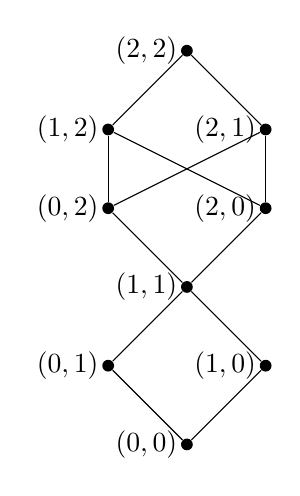
\begin{tikzpicture}
		\draw (0,0) node [left] (A) {$(0,0)$};
		\draw (-1,1) node [left] (B) {$(0,1)$};
		\draw (1,1) node [left] (C) {$(1,0)$};
		\draw (0,2) node [left] (D) {$(1,1)$};
		\draw (-1,3) node [left] (E) {$(0,2)$};
		\draw (1,3) node [left] (F) {$(2,0)$};
		\draw (-1,4) node [left] (G) {$(1,2)$};
		\draw (1,4) node [left] (H) {$(2,1)$};
		\draw (0,5) node [left] (I) {$(2,2)$};
		\draw node at (0,0) [circle,fill,inner sep=1.5pt] (A') {};
		\draw node at (-1,1) [circle,fill,inner sep=1.5pt] (B') {};
		\draw node at (1,1) [circle,fill,inner sep=1.5pt] (C') {};
		\draw node at (0,2) [circle,fill,inner sep=1.5pt] (D') {};
		\draw node at (-1,3) [circle,fill,inner sep=1.5pt] (E') {};
		\draw node at (1,3) [circle,fill,inner sep=1.5pt] (F') {};
		\draw node at (-1,4) [circle,fill,inner sep=1.5pt] (G') {};
		\draw node at (1,4) [circle,fill,inner sep=1.5pt] (H') {};
		\draw node at (0,5) [circle,fill,inner sep=1.5pt] (I') {};
		\draw (A') -- (B');
		\draw (A') -- (C');
		\draw (B') -- (D');
		\draw (C') -- (D');
		\draw (D') -- (E');
		\draw (D') -- (F');
		\draw (E') -- (G');
		\draw (E') -- (H');
		\draw (F') -- (G');
		\draw (F') -- (H');
		\draw (G') -- (I');
		\draw (H') -- (I');
	\end{tikzpicture}
\end{center}

\section*{Q.14}

\subsection*{(a)}

The maximal elements are $l$ and $m$.

\subsection*{(b)}

The minimal elements are $a$, $b$, and $c$.

\subsection*{(c)}

No.
There is no greatest element.

\subsection*{(d)}

No.
There is no least element.

\subsection*{(e)}

The upper bounds of $\{a,b,c\}$ are $k$, $l$, and $m$.

\subsection*{(f)}

The least upper bound of $\{a,b,c\}$ is $k$.

\subsection*{(g)}

The lower bound does not exist.

\subsection*{(h)}

The greatest lower bound does not exist.
\end{document}